\documentclass[12pt, a4paper]{article}
\usepackage[utf8]{inputenc}
\usepackage[T1]{fontenc}
\usepackage[brazil]{babel}
\usepackage{geometry}
\geometry{a4paper, margin=1.5cm, top=1.5cm, bottom=1.5cm}
\usepackage{booktabs}
\usepackage{tikz}
\usepackage{float}
\usepackage{amsmath}
\usepackage{multirow}
\usepackage{array}
\usepackage{xcolor}
\usepackage{listings}
\usepackage{caption}
\usepackage{hyperref}
\usepackage{amssymb}
\usepackage{microtype}

% fonte similar a Verdana (sans-serif Helvetica)
\usepackage{helvet}
\renewcommand{\familydefault}{\sfdefault}

% estilo dos trechos de codigo
\definecolor{codegray}{rgb}{0.5,0.5,0.5}
\definecolor{codegreen}{rgb}{0.1,0.5,0.1}
\definecolor{codeblue}{rgb}{0.1,0.1,0.6}
\definecolor{codebg}{rgb}{0.97,0.97,0.97}
\lstset{
    language=C,
    basicstyle=\ttfamily\footnotesize,
    keywordstyle=\color{codeblue}\bfseries,
    commentstyle=\color{codegreen},
    numberstyle=\tiny\color{codegray},
    backgroundcolor=\color{codebg},
    numbers=left,
    frame=single,
    breaklines=true,
    showstringspaces=false,
    tabsize=4,
    captionpos=b,
    morekeywords={mtype, pragma, omp, task, depend, single, parallel, taskwait},
    literate={á}{{\'a}}1 {é}{{\'e}}1 {í}{{\'i}}1 {ó}{{\'o}}1 {ú}{{\'u}}1
             {ã}{{\~a}}1 {õ}{{\~o}}1 {ç}{{\c{c}}}1 {ê}{{\^e}}1 {â}{{\^a}}1
}
\renewcommand{\lstlistingname}{Código}

\hypersetup{colorlinks=true, linkcolor=black, urlcolor=blue}

% Ajuste fino de espacamento de titulos e floats para rigor de 8 paginas
\usepackage{titlesec}
\titlespacing*{\section}{0pt}{6pt plus 1pt minus 1pt}{3pt plus 1pt minus 1pt}
\titlespacing*{\subsection}{0pt}{4pt plus 1pt minus 1pt}{2pt plus 1pt minus 1pt}
\setlength{\textfloatsep}{5pt plus 2pt minus 2pt}
\setlength{\intextsep}{5pt plus 2pt minus 2pt}
\setlength{\floatsep}{5pt plus 2pt minus 2pt}
\setlength{\parskip}{2pt plus 1pt minus 1pt}
\captionsetup{skip=3pt}

\title{\vspace{-1.2cm}\textbf{Relatório Prático: Paralelização do Algoritmo LCS (OpenMP + MPI)}\vspace{-0.4cm}}
\author{Gabriel Henrique Polo (GRR20241558) \and Vinícius Gregorio Fucci (GRR20241272)}
\date{\vspace{-0.3cm}Novembro de 2026 -- CI1316: Programação Paralela (DINF/UFPR)\vspace{-0.6cm}}

\begin{document}
\maketitle

\section{Introdução}
\label{sec:introducao}

Dado o kernel do algoritmo sequencial para resolver o problema da Maior Subsequência Comum (\textit{Longest Common Subsequence} -- LCS) baseado em programação dinâmica clássica $\mathcal{O}(M \times N)$ (Código~\ref{lst:kernel_seq}), o objetivo deste trabalho é paralelizar esta computação utilizando os paradigmas de memória compartilhada (\textbf{OpenMP}), memória distribuída (\textbf{MPI}) e de forma \textbf{híbrida} (\textbf{MPI + OpenMP}), analisando o desempenho e os \textit{speedups} obtidos na arquitetura multicore da servidora \textit{duo} (AMD Ryzen 9 5950X, 16 núcleos físicos).

\begin{lstlisting}[caption={Kernel sequencial do algoritmo LCS em linguagem C.}, label={lst:kernel_seq}]
int LCS(mtype **scoreMatrix, int sizeA, int sizeB, char *seqA, char *seqB) {
    int i, j;
    for (i = 1; i < sizeB + 1; i++) {
        for (j = 1; j < sizeA + 1; j++) {
            if (seqA[j - 1] == seqB[i - 1]) {
                scoreMatrix[i][j] = scoreMatrix[i - 1][j - 1] + 1;
            } else {
                scoreMatrix[i][j] = max(scoreMatrix[i - 1][j], 
                                        scoreMatrix[i][j - 1]);
            }
        }
    }
    return scoreMatrix[sizeB][sizeA];
}
\end{lstlisting}

\section{Estratégias de Paralelização}
\label{sec:paralelizacao}

\subsection{Evolução da Estratégia de Paralelização}
\label{sec:discussao_inicial}

A abordagem inicial avaliada para explorar a dependência em \textit{wavefront} consistiu em avançar diagonalmente pela matriz utilizando apenas 2 \textit{threads}: uma encarregada de computar a linha horizontal e a outra a coluna vertical até a posição $(i, j)$ da diagonal (Figura~\ref{fig:estrategia_openmp}a). No entanto, essa estratégia revelou dois gargalos determinantes: a concorrência fica estritamente limitada a 2 \textit{threads} e o cálculo da coluna quebra a contiguidade de memória em C (\textit{row-major}), gerando um volume excessivo de \textit{cache misses}.

Para superar essas restrições, a solução adotada foi a \textbf{decomposição 2D em blocos} (\textit{tiling}) de tamanho fixo $\texttt{BLOCK\_SIZE} \times \texttt{BLOCK\_SIZE}$. Cada bloco é processado sequencialmente linha a linha por uma \textit{thread}, garantindo localidade espacial na cache L1d e permitindo que múltiplos blocos ao longo das anti-diagonais sejam escalonados simultaneamente entre muitos núcleos (Figura~\ref{fig:estrategia_openmp}b).

\subsection{Versão OpenMP: Decomposição em Blocos 2D}
\label{sec:openmp}

Para minimizar a sobrecarga de sincronização e manter alta localidade de referência, a matriz é dividida em blocos de $\texttt{BLOCK\_SIZE} \times \texttt{BLOCK\_SIZE}$ ($512 \times 512$). Internamente, cada bloco é processado sequencialmente linha a linha, favorecendo o \textit{hardware prefetcher} e residindo integralmente na cache da CPU.

O paralelismo ocorre entre blocos via tarefas dependentes (\texttt{\#pragma omp task depend(in: ...) depend(out: ...)}). A thread principal (\texttt{\#pragma omp single}) percorre a grade e despacha as tarefas ao escalonador do OpenMP, que gerencia dinamicamente o Grafo Acíclico Dirigido (DAG). Utiliza-se \textit{padding} na matriz de sincronização (\texttt{sync\_matrix}) para eliminar desvios condicionais nas bordas (Figura~\ref{fig:estrategia_openmp}c).

\begin{figure}[H]
\centering
\begin{minipage}[b]{0.31\textwidth}
\centering
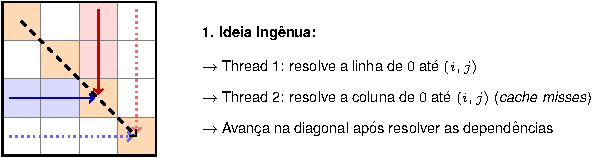
\includegraphics[width=\linewidth]{images/ideia_ingenua.pdf}
\caption*{(a) 2 \textit{threads} (ingênua).}
\end{minipage}\hfill
\begin{minipage}[b]{0.31\textwidth}
\centering
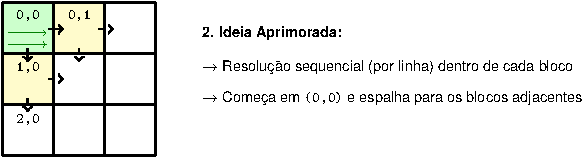
\includegraphics[width=\linewidth]{images/ideia_blocos.pdf}
\caption*{(b) Decomposição 2D.}
\end{minipage}\hfill
\begin{minipage}[b]{0.34\textwidth}
\centering
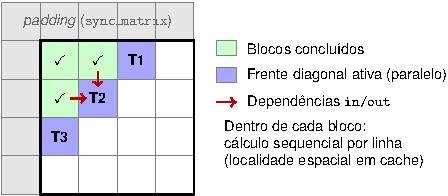
\includegraphics[width=\linewidth]{images/omp_wavefront.pdf}
\caption*{(c) Avanço diagonal com \textit{padding}.}
\end{minipage}
\caption{Evolução da paralelização em memória compartilhada (OpenMP): (a) restrição a 2 \textit{threads}; (b) blocos 2D escaláveis; (c) avanço diagonal com tarefas dependentes e \textit{padding}.}
\label{fig:estrategia_openmp}
\end{figure}

\subsection{Versão MPI: Decomposição 1D com Pipeline de Chunks}
\label{sec:mpi}

Na arquitetura de memória distribuída (MPI), as $M$ linhas da sequência B são particionadas horizontalmente em faixas contíguas balanceadas ($\lfloor M/P \rfloor$ linhas por processo). O processo de rank $0$ lê os arquivos e difunde os dados via \texttt{MPI\_Bcast}. 

Para evitar a serialização que ocorreria caso cada processo calculasse toda a sua faixa antes de comunicar a borda inferior, o eixo das colunas é fatiado em \textbf{\textit{chunks}} de largura \texttt{CHUNK\_SIZE} ($1024$), estabelecendo um \textbf{\textit{pipeline} de mensagens} (Figura~\ref{fig:mpi_hibrido_pipeline}a). O processo \texttt{rank} recebe do vizinho superior (\texttt{rank - 1}) a borda do \textit{chunk} atual via \texttt{MPI\_Recv}, processa suas linhas, transmite a última linha calculada ao vizinho inferior via \texttt{MPI\_Send} e avança imediatamente para o próximo \textit{chunk}, permitindo concorrência em estágios defasados do pipeline.

\subsection{Versão Híbrida: MPI + OpenMP em Dois Níveis}
\label{sec:hibrido}

A versão híbrida une os dois modelos hierarquicamente: no nível macro, o MPI gerencia o pipeline de \textit{chunks} entre processos; no nível micro, o OpenMP paraleliza o interior de cada \textit{chunk} em tarefas 2D. 

\begin{figure}[H]
\centering
\begin{minipage}[b]{0.45\textwidth}
\centering
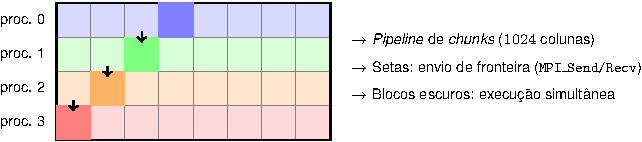
\includegraphics[height=2.2cm]{images/mpi_pipeline.pdf}
\caption*{(a) \textit{Pipeline} de \textit{chunks} no MPI.}
\end{minipage}\hfill
\begin{minipage}[b]{0.52\textwidth}
\centering
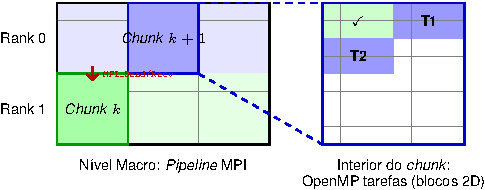
\includegraphics[height=2.2cm]{images/hibrido_arquitetura.pdf}
\caption*{(b) Híbrido: blocos OpenMP no \textit{chunk}.}
\end{minipage}
\caption{Modelos de execução distribuída e híbrida: (a) pipeline MPI; (b) tarefas OpenMP no \textit{chunk}.}
\label{fig:mpi_hibrido_pipeline}
\end{figure}

A comunicação usa \texttt{MPI\_THREAD\_FUNNELED}, assegurando que apenas a thread principal execute chamadas MPI fora de regiões paralelas. Como a largura do \textit{chunk} é $1024$ e o bloco OpenMP é $512$, há no máximo $\lceil 1024/512 \rceil = 2$ blocos na anti-diagonal por \textit{chunk}, limitando o paralelismo útil a 2 threads/processo e explicando a saturação do híbrido com mais threads.

\subsection{Otimização de Memória (\texttt{--mem-opt})}
\label{sec:memoria}

Na formulação ingênua com matriz completa (\texttt{--full-matrix}), o consumo de memória escala quadraticamente ($\mathcal{O}(N \cdot M)$). Para matrizes de grande porte ($100.000^2$ a $320.000^2$), essa alocação exigiria de 40 GiB a centenas de gigabytes de RAM, além de transformar a execução em um problema estritamente limitado pela largura de banda da memória (\textit{memory-bound}).

Como o objetivo é obter apenas o \textit{score} escalar final (e não o alinhamento completo), as células internas podem ser descartadas à medida que o cálculo diagonal em blocos avança:
\begin{itemize}
    \item \textbf{Sequencial:} Mantém apenas dois vetores de linha alternados (\texttt{prev\_row} e \texttt{curr\_row}), reduzindo o consumo para $\mathcal{O}(N)$.
    \item \textbf{OpenMP:} Armazena apenas os vetores de fronteira (\texttt{horiz\_borders} e \texttt{vert\_borders}) entre blocos. Cada tarefa aloca um buffer local de $513 \times 513$ elementos na pilha/cache, computa o miolo e grava de volta apenas a última linha e coluna.
    \item \textbf{MPI:} Cada processo mantém apenas dois vetores de tamanho $\texttt{CHUNK\_SIZE} + 1$ e um vetor vertical \texttt{left\_border} para a fronteira entre \textit{chunks}. Isso induz um \textbf{\textit{cache blocking}} ideal: duas linhas de 1024 posições ocupam 2 a 4 KiB, residindo integralmente na cache L1d (32 KiB).
\end{itemize}
Essa otimização viabiliza matrizes gigantescas (como Q7 de $160.000^2$ e Q8 de $320.000^2$) e elimina a contenção no barramento de memória.

\section{Ambiente de Execução e Metodologia}
\label{sec:ambiente}

Todos os experimentos foram conduzidos na servidora \textit{duo} do Departamento de Informática (DINF/UFPR). A Tabela~\ref{tab:cpu} sumariza as especificações do ambiente de hardware, software e os parâmetros operacionais estipulados.

\begin{table}[H]
\centering
\small
\caption{Configuração do ambiente e parâmetros de execução na servidora \textit{duo}.}
\label{tab:cpu}
\begin{tabular}{@{}ll@{}}
\toprule
\textbf{Parâmetro / Componente} & \textbf{Especificação / Valor Adotado} \\ \midrule
Processador & AMD Ryzen 9 5950X (1 soquete, 16 núcleos físicos / 32 threads lógicas) \\
Microarquitetura & Zen 3 (homogênea, sem divisão de núcleos P e E) \\
Frequência / Turbo Boost & Habilitado pelo firmware (estável em 3{,}6--4{,}7 GHz via telemetria contínua) \\
Governador DVFS & Padrão do sistema operacional (sem privilégio root para alteração) \\
Caches & L1d: 32 KiB/núcleo $\cdot$ L2: 512 KiB/núcleo $\cdot$ L3: $2 \times 32$ MiB compartilhada \\
Memória RAM & 125 GiB DDR4 \\
Sistema Operacional & Ubuntu 24.04 LTS (kernel Linux 6.8.0-49-generic) \\
Compilador & \texttt{gcc} 13.3.0 com flags de otimização máxima \texttt{-O3 -fopenmp} \\
OpenMPI & OpenMPI 5.0.x (ambiente Conda), comunicação intranó (\texttt{--mca btl \^{}tcp}) \\
Afinidade de CPU & \texttt{OMP\_PROC\_BIND=close}, \texttt{OMP\_PLACES=cores} (isolamento nos 16 núcleos físicos) \\
Amostragem Estatística & \textbf{20 repetições} por configuração com média e desvio padrão \\ \bottomrule
\end{tabular}
\end{table}

\subsection{Tipagem Dinâmica da Matriz e Recompilação Automática}
\label{sec:tipagem}

A matriz armazena inteiros do tipo \texttt{mtype} (\texttt{macros.h}). Para entradas com dimensão até $65.535$, compila-se com \texttt{uint16\_t} (2 bytes, alvo \texttt{make u16}), reduzindo a pegada de cache pela metade. Para dimensões superiores ($N, M \ge 65.535$), é obrigatório o uso de \texttt{uint32\_t} (\texttt{-DMTYPE\_32}, alvo \texttt{make u32}) para evitar \textit{overflow}. 

O script de automação dos experimentos (\texttt{run\_experiment.py}) gerencia essa transição de forma autônoma: ao detectar que o próximo caso de teste pertence a uma categoria de grande porte ou giga, ele aciona a recompilação imediata dos binários para o modo apropriado antes de iniciar as execuções.

\section{Entradas e Granularidade de Blocos}
\label{sec:entradas}

Para validar a corretude das implementações paralelas e avaliar diferentes regimes de casamento de caracteres e desvios condicionais, as entradas foram geradas sinteticamente via \texttt{generate\_input.py} combinando 5 padrões conceituais (Tabela~\ref{tab:padroes}).

\begin{table}[H]
\centering
\small
\caption{Padrões de caracteres e o score analítico esperado.}
\label{tab:padroes}
\begin{tabular}{@{}llll@{}}
\toprule
\textbf{Padrão} & \textbf{Sequência A} & \textbf{Sequência B} & \textbf{Score Esperado} \\ \midrule
\texttt{p1} & \texttt{"abcd"} repetido & \texttt{"bcda"} repetido & $\min(N,M) - 1$ \\
\texttt{p2} & \texttt{"a"} repetido & \texttt{"b"} repetido & $0$ \\
\texttt{p3} & \texttt{"abcd"} repetido & \texttt{"defg"} repetido & $\min(N,M)/4$ \\
\texttt{p4} & \texttt{"triviall"} repetido & \texttt{"triviall"} repetido & $\min(N,M)$ \\
\texttt{random} & Bytes pseudo-aleatórios & Bytes pseudo-aleatórios & $\approx 0{,}84 \min(N,M)$ (empírico) \\ \bottomrule
\end{tabular}
\end{table}

\subsection{Famílias de Matrizes e Parâmetros dos Ladrilhos}

A Tabela~\ref{tab:familias_entradas} sintetiza o conjunto de matrizes avaliadas, abrangendo diferentes volumes, proporções de aspecto e restrições de memória.

\begin{table}[H]
\centering
\footnotesize
\caption{Famílias de entradas, dimensões, padrões de caracteres e modos avaliados.}
\label{tab:familias_entradas}
\resizebox{\textwidth}{!}{%
\begin{tabular}{@{}llcc@{}}
\toprule
\textbf{Família / Casos} & \textbf{Dimensões ($M \times N$)} & \textbf{Padrões Avaliados} & \textbf{Modos Suportados} \\ \midrule
enunciado / quebrado & $10 \times 7$ / $827 \times 827$ & fixo / \texttt{p1} & \texttt{--full-matrix}, \texttt{--mem-opt} \\
Quadradas: Q1 a Q6 & $1.000^2$ até $100.000^2$ & \texttt{p1}, \texttt{p2}, \texttt{p3}, \texttt{p4}, \texttt{random} & \texttt{--full-matrix}, \texttt{--mem-opt} \\
Quadradas: Q7 e Q8 & $160.000^2$ e $320.000^2$ & Q7: todos (5); Q8: \texttt{p1} & apenas \texttt{--mem-opt} (giga) \\
Retangulares: R1 a R3 & $80k \times \{40, 20, 10\}k$ (e inv.) & todos (5) por variante & \texttt{--full-matrix}, \texttt{--mem-opt} \\
Retangulares: R4 a R6 & $160k \times \{80, 40, 20\}k$ (e inv.) & \texttt{p1} (direto e inv.) & apenas \texttt{--mem-opt} (giga) \\ \bottomrule
\end{tabular}%
}
\end{table}

Quanto à granularidade dos blocos, adotou-se \texttt{BLOCK\_SIZE} = \textbf{512} no OpenMP (definido empiricamente na Seção~\ref{sec:blocksize}) e \texttt{CHUNK\_SIZE} = \textbf{1024} no MPI (escolha de projeto para balancear latência e vazão no pipeline).

\section{Resultados Experimentais}
\label{sec:resultados}

Apresentamos a seguir os resultados consolidados obtidos na servidora \textit{duo}. Todas as métricas reportadas representam médias aritméticas de \textbf{20 repetições por configuração}. O \textit{speedup} adotado em todas as tabelas é o \textbf{speedup real (absoluto)}, calculado como a razão entre o tempo sequencial de referência ($\overline{T}_{seq}$) e o tempo da respectiva versão paralela com $p$ núcleos:
\begin{equation}
S(p) = \frac{\overline{T}_{seq}}{\overline{T}_{par}(p)}, \quad \text{com eficiência } E(p) = \frac{S(p)}{p}
\label{eq:speedup_real}
\end{equation}
Sempre que viável (entradas até Q6 e R3), a base do modo \texttt{--full-matrix} foi o tempo do programa sequencial original (\texttt{lcs\_seq} com matriz completa). Para as entradas gigantes (Q7, Q8 e R4 a R6), onde a matriz completa exigiria centenas de gigabytes excedendo a RAM física, a versão clássica foi inviabilizada; nesses casos, a referência sequencial $\overline{T}_{seq}$ no modo \texttt{--mem-opt} adota a execução sequencial otimizada em memória (ou $T(1)$) como base.

\subsection{Definição Experimental do \texttt{BLOCK\_SIZE}}
\label{sec:blocksize}

Para definir empiricamente a granularidade das tarefas OpenMP, executou-se uma varredura com os valores 64, 128, 256 e 512 através de \texttt{run\_test.py}. A Tabela~\ref{tab:blocksize} exibe o speedup alcançado.

\begin{table}[H]
\centering
\small
\caption{\textit{Speedup} da versão OpenMP em função do \texttt{BLOCK\_SIZE}.}
\label{tab:blocksize}
\begin{tabular}{@{}llccccc@{}}
\toprule
\textbf{Entrada} & \textbf{Modo} & \textbf{\textit{Threads}} & \textbf{64} & \textbf{128} & \textbf{256} & \textbf{512} \\ \midrule
\multirow{3}{*}{Q4\_random} & \multirow{3}{*}{\texttt{--full-matrix}} 
   & 4  & 1{,}55 & 1{,}77 & 1{,}90 & \textbf{2{,}13} \\
 & & 8  & 1{,}83 & 2{,}45 & 2{,}49 & \textbf{2{,}74} \\
 & & 16 & 3{,}10 & 2{,}84 & 3{,}05 & \textbf{3{,}21} \\ \cmidrule(l){2-7}
\multirow{3}{*}{Q4\_random} & \multirow{3}{*}{\texttt{--mem-opt}} 
   & 4  & 1{,}93 & 2{,}85 & 3{,}43 & \textbf{3{,}62} \\
 & & 8  & 2{,}47 & 4{,}58 & 6{,}02 & \textbf{6{,}50} \\
 & & 16 & 3{,}07 & 9{,}26 & 10{,}73 & \textbf{11{,}39} \\ \midrule
\multirow{2}{*}{Q5\_random} & \multirow{2}{*}{\texttt{--mem-opt}} 
   & 8  & 2{,}02 & 3{,}09 & 3{,}76 & \textbf{4{,}00} \\
 & & 16 & 2{,}87 & 5{,}11 & 7{,}05 & \textbf{7{,}40} \\ \bottomrule
\end{tabular}
\end{table}

O tamanho de bloco 512 superou os demais em todas as configurações. Blocos pequenos (como 64) geram dezenas de milhares de tarefas, sobrecarregando o escalonador do OpenMP com custo de despacho. O valor 512 amortiza o despacho e reside perfeitamente nas caches da CPU.

\subsection{Tempos Sequenciais e Fração Não-Paralelizável}
\label{sec:fracao_seq}

A Tabela~\ref{tab:tempo_seq} lista o tempo total sequencial ($\overline{T}_{seq}$) e decompõe a execução na porcentagem estritamente sequencial ($s = T_{puramente\_seq} / T_{total}$, associada a I/O com \texttt{read\_seq} e alocações dinâmicas) e na porcentagem paralelizável correspondente ($1 - s$).

\begin{table}[H]
\centering
\footnotesize
\caption{Tempos sequenciais médios e porcentagens de tempo sequencial ($s$) e paralelizável ($1-s$).}
\label{tab:tempo_seq}
\resizebox{\textwidth}{!}{%
\begin{tabular}{@{}ll|ccc|ccc@{}}
\toprule
 & & \multicolumn{3}{c|}{\textbf{Matriz Completa (\texttt{--full-matrix})}} 
   & \multicolumn{3}{c}{\textbf{Otimizado (\texttt{--mem-opt})}} \\
\textbf{Caso} & \textbf{Dimensões} & $\overline{T}_{seq}$ (s) & \textbf{\% Seq} & \textbf{\% Par} & $\overline{T}_{seq}$ (s) & \textbf{\% Seq} & \textbf{\% Par} \\ \midrule
enunciado       & $10 \times 7$          & 0{,}0000 & 77{,}7\% & 22{,}3\% & 0{,}0000 & 46{,}5\% & 53{,}5\% \\
número quebrado & $827 \times 827$       & 0{,}0011 & 57{,}1\% & 42{,}9\% & 0{,}0005 & 3{,}7\%  & 96{,}3\% \\
Q1              & $1.000^2$             & 0{,}0019 & 48{,}2\% & 51{,}8\% & 0{,}0013 & 2{,}3\%  & 97{,}7\% \\
Q2              & $10.000^2$            & 0{,}1710 & 14{,}0\% & 86{,}0\% & 0{,}1072 & 0{,}16\% & 99{,}84\% \\
Q3              & $20.000^2$            & 0{,}6813 & 9{,}8\%  & 90{,}2\% & 0{,}4292 & 0{,}07\% & 99{,}93\% \\
Q4              & $40.000^2$            & 2{,}7189 & 7{,}9\%  & 92{,}1\% & 1{,}7173 & 0{,}04\% & 99{,}96\% \\
Q5              & $80.000^2$            & 13{,}1827& 9{,}5\%  & 90{,}5\% & 4{,}1488 & 0{,}04\% & 99{,}96\% \\
Q6              & $100.000^2$           & 20{,}3669& 9{,}3\%  & 90{,}7\% & 6{,}5041 & 0{,}04\% & 99{,}96\% \\
Q7              & $160.000^2$           & --       & --       & --       & 16{,}5260& 0{,}01\% & 99{,}99\% \\
Q8              & $320.000^2$           & --       & --       & --       & 74{,}5281& 0{,}01\% & 99{,}99\% \\
R1              & $80k \times 40k$ (2:1) & 5{,}7452 & 6{,}5\%  & 93{,}5\% & 3{,}8438 & 0{,}03\% & 99{,}97\% \\
R1\_inv         & $40k \times 80k$ (1:2) & 5{,}4337 & 7{,}7\%  & 92{,}3\% & 3{,}4334 & 0{,}03\% & 99{,}97\% \\
R2              & $80k \times 20k$ (4:1) & 2{,}8844 & 6{,}6\%  & 93{,}4\% & 1{,}9235 & 0{,}04\% & 99{,}96\% \\
R2\_inv         & $20k \times 80k$ (1:4) & 2{,}7521 & 10{,}0\% & 90{,}0\% & 1{,}7141 & 0{,}05\% & 99{,}95\% \\
R3              & $80k \times 10k$ (8:1) & 1{,}4682 & 7{,}2\%  & 92{,}8\% & 0{,}9610 & 0{,}07\% & 99{,}93\% \\
R3\_inv         & $10k \times 80k$ (1:8) & 1{,}3825 & 13{,}5\% & 86{,}5\% & 0{,}8581 & 0{,}08\% & 99{,}92\% \\
R4              & $160k \times 80k$ (2:1)& --       & --       & --       & 9{,}3322 & 0{,}03\% & 99{,}97\% \\
R4\_inv         & $80k \times 160k$ (1:2)& --       & --       & --       & 9{,}3346 & 0{,}03\% & 99{,}97\% \\
R5              & $160k \times 40k$ (4:1)& --       & --       & --       & 4{,}6779 & 0{,}04\% & 99{,}96\% \\
R5\_inv         & $40k \times 160k$ (1:4)& --       & --       & --       & 4{,}6502 & 0{,}04\% & 99{,}96\% \\
R6              & $160k \times 20k$ (8:1)& --       & --       & --       & 2{,}3358 & 0{,}03\% & 99{,}97\% \\
R6\_inv         & $20k \times 160k$ (1:8)& --       & --       & --       & 2{,}0905 & 0{,}03\% & 99{,}97\% \\ \bottomrule
\end{tabular}%
}
\end{table}

\subsection{Estimativa Teórica pela Lei de Amdahl}
\label{sec:amdahl}

Com base na fração puramente sequencial $s$ medida, a Lei de Amdahl estabelece o speedup teórico:
\begin{equation}
S_{Amdahl}(p) = \frac{1}{s + \frac{1 - s}{p}}, \quad \text{com limite assintótico } S_{max} = \lim_{p \to \infty} S_{Amdahl}(p) = \frac{1}{s}
\label{eq:amdahl}
\end{equation}

A Tabela~\ref{tab:amdahl} apresenta as projeções teóricas. Na matriz completa, o custo de alocação impõe $s \approx 8\% \text{ a } 14\%$, limitando o teto teórico a no máximo $\approx 10\times \text{ a } 12{,}7\times$. Em contrapartida, no modo otimizado (\texttt{--mem-opt}), a ausência de matriz interna reduz $s$ para $<0{,}1\%$, elevando o teto teórico para centenas ou milhares de vezes.

\begin{table}[H]
\centering
\small
\caption{Speedup máximo teórico pela Lei de Amdahl em função do número de núcleos ($p$).}
\label{tab:amdahl}
\begin{tabular}{@{}lccccccc@{}}
\toprule
\textbf{Caso / Modo} & \textbf{Fração Seq. ($s$)} & \textbf{$p=2$} & \textbf{$p=4$} & \textbf{$p=8$} & \textbf{$p=16$} & \textbf{$p=32$} & \textbf{$p \to \infty$ ($1/s$)} \\ \midrule
Q2 (\texttt{full-matrix}) & $14{,}00\%$ & 1{,}75 & 2{,}82 & 4{,}04 & 5{,}16 & 6{,}04 & \textbf{7{,}14$\times$} \\
Q3 (\texttt{full-matrix}) & $9{,}80\%$  & 1{,}82 & 3{,}09 & 4{,}74 & 6{,}48 & 7{,}98 & \textbf{10{,}20$\times$} \\
Q4 (\texttt{full-matrix}) & $7{,}90\%$  & 1{,}85 & 3{,}23 & 5{,}15 & 7{,}32 & 9{,}38 & \textbf{12{,}66$\times$} \\
Q6 (\texttt{full-matrix}) & $9{,}30\%$  & 1{,}83 & 3{,}13 & 4{,}85 & 6{,}68 & 8{,}29 & \textbf{10{,}75$\times$} \\ \midrule
Q2 (\texttt{--mem-opt})   & $0{,}16\%$  & 2{,}00 & 3{,}98 & 7{,}91 & 15{,}62 & 30{,}46 & \textbf{625$\times$} \\
Q4 (\texttt{--mem-opt})   & $0{,}04\%$  & 2{,}00 & 4{,}00 & 7{,}98 & 15{,}90 & 31{,}60 & \textbf{2.500$\times$} \\
Q7 e Q8 (\texttt{--mem-opt}) & $0{,}01\%$  & 2{,}00 & 4{,}00 & 7{,}99 & 15{,}98 & 31{,}90 & \textbf{10.000$\times$} \\ \bottomrule
\end{tabular}
\end{table}

\subsection{Speedup e Eficiência no Modo Matriz Completa (\texttt{--full-matrix})}

A Tabela~\ref{tab:res_full} apresenta o \textit{speedup} e a Tabela~\ref{tab:ef_full} reporta a eficiência correspondente ($E_p = S_p / p$) para a versão com matriz completa.

\begin{table}[H]
\centering
\caption{Speedup médio das 20 repetições e de todos os 5 padrões para cada entrada no modo \texttt{--full-matrix}.}
\label{tab:res_full}
\resizebox{\textwidth}{!}{%
\begin{tabular}{@{}l|ccccc|ccccc|cccccc@{}}
\toprule
 & \multicolumn{5}{c|}{\textbf{OpenMP (\textit{threads})}} 
 & \multicolumn{5}{c|}{\textbf{MPI (\textit{processos})}} 
 & \multicolumn{6}{c}{\textbf{Híbrido ($proc \times th$)}} \\
Caso & 1 & 2 & 4 & 8 & 16 & 1 & 2 & 4 & 8 & 16 & $2\times2$ & $2\times4$ & $4\times2$ & $2\times8$ & $4\times4$ & $8\times2$ \\ \midrule
enunciado       & \textbf{0{,}71} & 0{,}23 & 0{,}12 & 0{,}07 & 0{,}04 & 0{,}00 & \textbf{0{,}36} & 0{,}18 & 0{,}15 & 0{,}08 & \textbf{0{,}12} & 0{,}07 & 0{,}06 & 0{,}04 & 0{,}03 & 0{,}03 \\
número quebrado & \textbf{1{,}04} & 1{,}03 & 0{,}91 & 0{,}85 & 0{,}64 & 1{,}18 & 1{,}16 & 1{,}05 & \textbf{1{,}62} & 1{,}21 & 0{,}74 & \textbf{0{,}82} & 0{,}65 & 0{,}69 & 0{,}64 & 0{,}79 \\
Q1              & 1{,}00 & \textbf{1{,}01} & 0{,}98 & 0{,}91 & 0{,}72 & 1{,}09 & 1{,}07 & 1{,}00 & 0{,}91 & \textbf{1{,}14} & 0{,}74 & \textbf{0{,}82} & 0{,}68 & 0{,}73 & 0{,}69 & 0{,}58 \\
Q2              & 0{,}81 & 1{,}45 & 2{,}20 & 2{,}87 & \textbf{3{,}13} & 0{,}85 & 1{,}39 & 1{,}99 & 2{,}54 & \textbf{2{,}65} & 1{,}62 & 1{,}73 & 2{,}14 & 1{,}69 & 2{,}35 & \textbf{2{,}55} \\
Q3              & 0{,}78 & 1{,}44 & 2{,}31 & 3{,}18 & \textbf{3{,}93} & 0{,}86 & 1{,}52 & 2{,}41 & 3{,}38 & \textbf{4{,}16} & 1{,}88 & 1{,}94 & 2{,}77 & 1{,}91 & 2{,}92 & \textbf{3{,}56} \\
Q4              & 0{,}76 & 1{,}41 & 2{,}33 & 3{,}24 & \textbf{4{,}03} & 0{,}86 & 1{,}61 & 2{,}72 & 3{,}98 & \textbf{5{,}18} & 2{,}04 & 2{,}09 & 3{,}27 & 2{,}07 & 3{,}36 & \textbf{4{,}38} \\
Q5              & 0{,}73 & 1{,}33 & 2{,}06 & 2{,}54 & \textbf{2{,}75} & 0{,}86 & 1{,}64 & 2{,}89 & 4{,}04 & \textbf{4{,}58} & 2{,}13 & 2{,}16 & 3{,}40 & 2{,}15 & 3{,}44 & \textbf{3{,}94} \\
Q6              & 0{,}72 & 1{,}32 & 2{,}05 & 2{,}53 & \textbf{2{,}73} & 0{,}86 & 1{,}64 & 2{,}91 & 4{,}10 & \textbf{4{,}64} & 2{,}15 & 2{,}18 & 3{,}45 & 2{,}15 & 3{,}48 & \textbf{3{,}99} \\
R1              & 0{,}74 & 1{,}41 & 2{,}36 & 3{,}44 & \textbf{4{,}32} & 0{,}85 & 1{,}59 & 2{,}75 & 4{,}06 & \textbf{5{,}32} & 2{,}14 & 2{,}17 & 3{,}49 & 2{,}17 & 3{,}56 & \textbf{4{,}66} \\
R1\_inv         & 0{,}75 & 1{,}39 & 2{,}30 & 3{,}20 & \textbf{3{,}95} & 0{,}85 & 1{,}59 & 2{,}72 & 3{,}95 & \textbf{5{,}11} & 2{,}09 & 2{,}13 & 3{,}37 & 2{,}13 & 3{,}46 & \textbf{4{,}48} \\
R2              & 0{,}75 & 1{,}48 & 2{,}44 & 3{,}54 & \textbf{4{,}60} & 0{,}86 & 1{,}53 & 2{,}45 & 3{,}34 & \textbf{4{,}17} & 1{,}98 & 2{,}05 & 2{,}96 & 2{,}03 & 3{,}09 & \textbf{3{,}75} \\
R2\_inv         & 0{,}78 & 1{,}42 & 2{,}28 & 3{,}11 & \textbf{3{,}94} & 0{,}86 & 1{,}52 & 2{,}44 & 3{,}31 & \textbf{4{,}08} & 1{,}94 & 2{,}02 & 2{,}88 & 2{,}00 & 3{,}03 & \textbf{3{,}65} \\
R3              & 0{,}80 & 1{,}57 & 2{,}60 & 3{,}80 & \textbf{4{,}84} & 0{,}85 & 1{,}39 & 2{,}01 & 2{,}48 & \textbf{2{,}77} & 1{,}71 & 1{,}80 & 2{,}29 & 1{,}79 & 2{,}48 & \textbf{2{,}68} \\
R3\_inv         & 0{,}78 & 1{,}41 & 2{,}21 & 3{,}02 & \textbf{3{,}68} & 0{,}85 & 1{,}38 & 1{,}97 & 2{,}42 & \textbf{2{,}70} & 1{,}65 & 1{,}76 & 2{,}21 & 1{,}74 & 2{,}40 & \textbf{2{,}56} \\ \bottomrule
\end{tabular}%
}
\end{table}

\begin{table}[H]
\centering
\caption{Eficiência ($E = S / p$) no modo \texttt{--full-matrix}.}
\label{tab:ef_full}
\resizebox{\textwidth}{!}{%
\begin{tabular}{@{}l|ccccc|ccccc|cccccc@{}}
\toprule
 & \multicolumn{5}{c|}{\textbf{OpenMP (\textit{threads})}} 
 & \multicolumn{5}{c|}{\textbf{MPI (\textit{processos})}} 
 & \multicolumn{6}{c}{\textbf{Híbrido ($total\_cores$)}} \\
Caso & 1 & 2 & 4 & 8 & 16 & 1 & 2 & 4 & 8 & 16 & 4 ($2\times2$) & 8 ($2\times4$) & 8 ($4\times2$) & 16 ($2\times8$) & 16 ($4\times4$) & 16 ($8\times2$) \\ \midrule
Q2 & \textbf{0{,}81} & 0{,}72 & 0{,}55 & 0{,}36 & 0{,}20 & \textbf{0{,}85} & 0{,}69 & 0{,}50 & 0{,}32 & 0{,}17 & \textbf{0{,}41} & 0{,}22 & 0{,}27 & 0{,}11 & 0{,}15 & 0{,}16 \\
Q3 & \textbf{0{,}78} & 0{,}72 & 0{,}58 & 0{,}40 & 0{,}25 & \textbf{0{,}86} & 0{,}76 & 0{,}60 & 0{,}42 & 0{,}26 & \textbf{0{,}47} & 0{,}24 & 0{,}35 & 0{,}12 & 0{,}18 & 0{,}22 \\
Q4 & \textbf{0{,}76} & 0{,}71 & 0{,}58 & 0{,}41 & 0{,}25 & \textbf{0{,}86} & 0{,}80 & 0{,}68 & 0{,}50 & 0{,}32 & \textbf{0{,}51} & 0{,}26 & 0{,}41 & 0{,}13 & 0{,}21 & 0{,}27 \\
Q5 & \textbf{0{,}73} & 0{,}66 & 0{,}52 & 0{,}32 & 0{,}17 & \textbf{0{,}86} & 0{,}82 & 0{,}72 & 0{,}51 & 0{,}29 & \textbf{0{,}53} & 0{,}27 & 0{,}43 & 0{,}13 & 0{,}21 & 0{,}25 \\
Q6 & \textbf{0{,}72} & 0{,}66 & 0{,}51 & 0{,}32 & 0{,}17 & \textbf{0{,}86} & 0{,}82 & 0{,}73 & 0{,}51 & 0{,}29 & \textbf{0{,}54} & 0{,}27 & 0{,}43 & 0{,}13 & 0{,}22 & 0{,}25 \\
R1 & \textbf{0{,}74} & 0{,}70 & 0{,}59 & 0{,}43 & 0{,}27 & \textbf{0{,}85} & 0{,}80 & 0{,}69 & 0{,}51 & 0{,}33 & \textbf{0{,}53} & 0{,}27 & 0{,}44 & 0{,}14 & 0{,}22 & 0{,}29 \\ \bottomrule
\end{tabular}%
}
\end{table}

\subsection{Speedup e Eficiência no Modo Otimizado de Memória (\texttt{--mem-opt})}

A Tabela~\ref{tab:res_memopt} lista o \textit{speedup} e a Tabela~\ref{tab:ef_memopt} a eficiência no modo otimizado de memória, cobrindo as matrizes gigantescas (Q7 e Q8) e os retângulos de grande escala (R1 a R6).

\begin{table}[H]
\centering
\caption{Speedup médio das 20 repetições e de todos os 5 padrões para cada entrada no modo \texttt{--mem-opt}.}
\label{tab:res_memopt}
\resizebox{\textwidth}{!}{%
\begin{tabular}{@{}l|ccccc|ccccc|cccccc@{}}
\toprule
 & \multicolumn{5}{c|}{\textbf{OpenMP (\textit{threads})}} 
 & \multicolumn{5}{c|}{\textbf{MPI (\textit{processos})}} 
 & \multicolumn{6}{c}{\textbf{Híbrido ($proc \times th$)}} \\
Caso & 1 & 2 & 4 & 8 & 16 & 1 & 2 & 4 & 8 & 16 & $2\times2$ & $2\times4$ & $4\times2$ & $2\times8$ & $4\times4$ & $8\times2$ \\ \midrule
enunciado       & \textbf{0{,}47} & 0{,}17 & 0{,}09 & 0{,}05 & 0{,}02 & \textbf{0{,}89} & 0{,}32 & 0{,}18 & 0{,}14 & 0{,}07 & \textbf{0{,}11} & 0{,}06 & 0{,}05 & 0{,}04 & 0{,}03 & 0{,}03 \\
número quebrado & \textbf{0{,}69} & 0{,}56 & 0{,}49 & 0{,}40 & 0{,}30 & \textbf{1{,}32} & 1{,}24 & 1{,}10 & 0{,}93 & 0{,}74 & 0{,}36 & \textbf{0{,}37} & 0{,}31 & 0{,}31 & 0{,}30 & 0{,}36 \\
Q1              & \textbf{0{,}80} & 0{,}80 & 0{,}74 & 0{,}66 & 0{,}52 & \textbf{1{,}38} & 1{,}33 & 1{,}22 & 1{,}08 & 0{,}90 & \textbf{0{,}57} & 0{,}57 & 0{,}51 & 0{,}51 & 0{,}48 & 0{,}43 \\
Q2              & 0{,}96 & 1{,}89 & 3{,}50 & 5{,}62 & \textbf{5{,}68} & 1{,}18 & 2{,}13 & 3{,}31 & 4{,}54 & \textbf{5{,}43} & 2{,}04 & 2{,}03 & 2{,}88 & 1{,}99 & 2{,}91 & \textbf{3{,}40} \\
Q3              & 0{,}96 & 1{,}91 & 3{,}68 & 6{,}57 & \textbf{10{,}38} & 1{,}17 & 2{,}23 & 3{,}90 & 6{,}11 & \textbf{8{,}05} & 2{,}27 & 2{,}27 & 3{,}66 & 2{,}22 & 3{,}67 & \textbf{5{,}11} \\
Q4              & 0{,}96 & 1{,}92 & 3{,}73 & 6{,}83 & \textbf{12{,}30} & 1{,}17 & 2{,}28 & 4{,}23 & 7{,}25 & \textbf{11{,}21} & 2{,}39 & 2{,}40 & 4{,}09 & 2{,}38 & 4{,}08 & \textbf{5{,}58} \\
Q5              & 0{,}53 & 1{,}05 & 2{,}05 & 3{,}69 & \textbf{6{,}96} & 1{,}19 & 2{,}34 & 4{,}41 & 7{,}77 & \textbf{13{,}25} & 1{,}49 & 1{,}53 & 1{,}96 & 1{,}51 & 1{,}98 & \textbf{2{,}15} \\
Q6              & 0{,}53 & 1{,}05 & 2{,}05 & 3{,}69 & \textbf{7{,}01} & 1{,}19 & 2{,}34 & 4{,}44 & 7{,}70 & \textbf{13{,}68} & 1{,}50 & 1{,}55 & 1{,}99 & 1{,}53 & 2{,}02 & \textbf{2{,}19} \\
Q7              & 0{,}53 & 1{,}05 & 2{,}03 & 3{,}64 & \textbf{6{,}98} & 1{,}18 & 2{,}33 & 4{,}46 & 7{,}76 & \textbf{14{,}08} & 1{,}54 & 1{,}58 & 2{,}03 & 1{,}57 & 2{,}05 & \textbf{2{,}22} \\
Q8              & 0{,}59 & 1{,}17 & 2{,}28 & 4{,}07 & \textbf{7{,}81} & 1{,}34 & 2{,}63 & 5{,}13 & 8{,}92 & \textbf{16{,}61} & 1{,}83 & 1{,}89 & 2{,}35 & 1{,}87 & 2{,}38 & \textbf{2{,}56} \\
R1 ($80k \times 40k$)   & 1{,}00 & 2{,}00 & 3{,}87 & 7{,}13 & \textbf{13{,}34} & 1{,}17 & 2{,}28 & 4{,}23 & 7{,}28 & \textbf{11{,}59} & 2{,}57 & 2{,}56 & 4{,}42 & 2{,}54 & 4{,}39 & \textbf{5{,}91} \\
R1\_inv ($40k \times 80k$) & 0{,}96 & 1{,}92 & 3{,}73 & 6{,}84 & \textbf{12{,}68} & 1{,}17 & 2{,}28 & 4{,}23 & 7{,}25 & \textbf{11{,}45} & 2{,}40 & 2{,}40 & 4{,}09 & 2{,}38 & 4{,}06 & \textbf{5{,}37} \\
R2 ($80k \times 20k$)   & 1{,}00 & 2{,}00 & 3{,}88 & 7{,}14 & \textbf{12{,}96} & 1{,}17 & 2{,}23 & 3{,}95 & 6{,}33 & \textbf{8{,}91} & 2{,}37 & 2{,}37 & 3{,}83 & 2{,}35 & 3{,}81 & \textbf{5{,}00} \\
R2\_inv ($20k \times 80k$) & 0{,}96 & 1{,}92 & 3{,}72 & 6{,}83 & \textbf{12{,}29} & 1{,}17 & 2{,}22 & 3{,}95 & 6{,}31 & \textbf{8{,}82} & 2{,}20 & 2{,}21 & 3{,}53 & 2{,}19 & 3{,}52 & \textbf{4{,}54} \\
R3 ($80k \times 10k$)   & 1{,}00 & 2{,}00 & 3{,}86 & 7{,}07 & \textbf{12{,}05} & 1{,}17 & 2{,}12 & 3{,}47 & 4{,}98 & \textbf{6{,}10} & 2{,}09 & 2{,}08 & 3{,}06 & 2{,}06 & 3{,}03 & \textbf{3{,}80} \\
R3\_inv ($10k \times 80k$) & 0{,}96 & 1{,}92 & 3{,}71 & 6{,}72 & \textbf{11{,}28} & 1{,}17 & 2{,}12 & 3{,}47 & 4{,}95 & \textbf{5{,}99} & 1{,}93 & 1{,}93 & 2{,}81 & 1{,}92 & 2{,}80 & \textbf{3{,}46} \\
R4 ($160k \times 80k$)  & 0{,}59 & 1{,}17 & 2{,}29 & 4{,}14 & \textbf{7{,}82} & 1{,}34 & 2{,}62 & 5{,}00 & 8{,}54 & \textbf{14{,}62} & 1{,}74 & 1{,}79 & 2{,}21 & 1{,}77 & 2{,}24 & \textbf{2{,}41} \\
R4\_inv ($80k \times 160k$)& 0{,}59 & 1{,}17 & 2{,}29 & 4{,}14 & \textbf{7{,}81} & 1{,}34 & 2{,}61 & 4{,}97 & 8{,}56 & \textbf{14{,}61} & 1{,}74 & 1{,}78 & 2{,}22 & 1{,}77 & 2{,}23 & \textbf{2{,}41} \\
R5 ($160k \times 40k$)  & 0{,}59 & 1{,}18 & 2{,}29 & 4{,}13 & \textbf{7{,}77} & 1{,}34 & 2{,}60 & 4{,}83 & 7{,}97 & \textbf{12{,}69} & 1{,}64 & 1{,}69 & 2{,}07 & 1{,}67 & 2{,}08 & \textbf{2{,}25} \\
R5\_inv ($40k \times 160k$)& 0{,}59 & 1{,}17 & 2{,}28 & 4{,}12 & \textbf{7{,}73} & 1{,}33 & 2{,}59 & 4{,}82 & 7{,}94 & \textbf{12{,}52} & 1{,}63 & 1{,}67 & 2{,}05 & 1{,}66 & 2{,}07 & \textbf{2{,}23} \\
R6 ($160k \times 20k$)  & 0{,}59 & 1{,}17 & 2{,}29 & 4{,}14 & \textbf{7{,}65} & 1{,}34 & 2{,}52 & 4{,}50 & 6{,}91 & \textbf{9{,}84} & 1{,}46 & 1{,}50 & 1{,}80 & 1{,}49 & 1{,}82 & \textbf{1{,}96} \\
R6\_inv ($20k \times 160k$)& 0{,}53 & 1{,}05 & 2{,}05 & 3{,}72 & \textbf{6{,}85} & 1{,}20 & 2{,}25 & 4{,}03 & 6{,}26 & \textbf{8{,}78} & 1{,}31 & 1{,}34 & 1{,}61 & 1{,}33 & 1{,}63 & \textbf{1{,}75} \\ \bottomrule
\end{tabular}%
}
\end{table}

\begin{table}[H]
\centering
\caption{Eficiência ($E = S / p$) no modo \texttt{--mem-opt}.}
\label{tab:ef_memopt}
\resizebox{\textwidth}{!}{%
\begin{tabular}{@{}l|ccccc|ccccc|cccccc@{}}
\toprule
 & \multicolumn{5}{c|}{\textbf{OpenMP (\textit{threads})}} 
 & \multicolumn{5}{c|}{\textbf{MPI (\textit{processos})}} 
 & \multicolumn{6}{c}{\textbf{Híbrido ($total\_cores$)}} \\
Caso & 1 & 2 & 4 & 8 & 16 & 1 & 2 & 4 & 8 & 16 & 4 ($2\times2$) & 8 ($2\times4$) & 8 ($4\times2$) & 16 ($2\times8$) & 16 ($4\times4$) & 16 ($8\times2$) \\ \midrule
Q2         & \textbf{0{,}96} & 0{,}94 & 0{,}87 & 0{,}70 & 0{,}36 & \textbf{1{,}18} & 1{,}06 & 0{,}83 & 0{,}57 & 0{,}34 & \textbf{0{,}51} & 0{,}25 & 0{,}36 & 0{,}12 & 0{,}18 & 0{,}21 \\
Q3         & \textbf{0{,}96} & 0{,}96 & 0{,}92 & 0{,}82 & 0{,}65 & \textbf{1{,}17} & 1{,}12 & 0{,}98 & 0{,}76 & 0{,}50 & \textbf{0{,}57} & 0{,}28 & 0{,}46 & 0{,}14 & 0{,}23 & 0{,}32 \\
Q4         & \textbf{0{,}96} & 0{,}96 & 0{,}93 & 0{,}85 & 0{,}77 & \textbf{1{,}17} & 1{,}14 & 1{,}06 & 0{,}91 & 0{,}70 & \textbf{0{,}60} & 0{,}30 & 0{,}51 & 0{,}15 & 0{,}25 & 0{,}35 \\
Q5         & \textbf{0{,}53} & 0{,}52 & 0{,}51 & 0{,}46 & 0{,}43 & \textbf{1{,}19} & 1{,}17 & 1{,}10 & 0{,}97 & 0{,}83 & \textbf{0{,}37} & 0{,}19 & 0{,}24 & 0{,}09 & 0{,}12 & 0{,}13 \\
Q6         & \textbf{0{,}53} & 0{,}53 & 0{,}51 & 0{,}46 & 0{,}44 & \textbf{1{,}19} & 1{,}17 & 1{,}11 & 0{,}96 & 0{,}86 & \textbf{0{,}38} & 0{,}19 & 0{,}25 & 0{,}10 & 0{,}13 & 0{,}14 \\
Q7         & \textbf{0{,}53} & 0{,}52 & 0{,}51 & 0{,}46 & 0{,}44 & \textbf{1{,}18} & 1{,}17 & 1{,}12 & 0{,}97 & 0{,}88 & \textbf{0{,}39} & 0{,}20 & 0{,}25 & 0{,}10 & 0{,}13 & 0{,}14 \\
Q8         & \textbf{0{,}59} & 0{,}59 & 0{,}57 & 0{,}51 & 0{,}49 & \textbf{1{,}34} & 1{,}31 & 1{,}28 & 1{,}12 & 1{,}04 & \textbf{0{,}46} & 0{,}24 & 0{,}29 & 0{,}12 & 0{,}15 & 0{,}16 \\
R1         & \textbf{1{,}00} & 1{,}00 & 0{,}97 & 0{,}89 & 0{,}83 & \textbf{1{,}17} & 1{,}14 & 1{,}06 & 0{,}91 & 0{,}72 & \textbf{0{,}64} & 0{,}32 & 0{,}55 & 0{,}16 & 0{,}27 & 0{,}37 \\
R1\_inv    & \textbf{0{,}96} & 0{,}96 & 0{,}93 & 0{,}85 & 0{,}79 & \textbf{1{,}17} & 1{,}14 & 1{,}06 & 0{,}91 & 0{,}72 & \textbf{0{,}60} & 0{,}30 & 0{,}51 & 0{,}15 & 0{,}25 & 0{,}34 \\
R4         & \textbf{0{,}59} & 0{,}59 & 0{,}57 & 0{,}52 & 0{,}49 & \textbf{1{,}34} & 1{,}31 & 1{,}25 & 1{,}07 & 0{,}91 & \textbf{0{,}43} & 0{,}22 & 0{,}28 & 0{,}11 & 0{,}14 & 0{,}15 \\
R4\_inv    & \textbf{0{,}59} & 0{,}59 & 0{,}57 & 0{,}52 & 0{,}49 & \textbf{1{,}34} & 1{,}31 & 1{,}24 & 1{,}07 & 0{,}91 & \textbf{0{,}43} & 0{,}22 & 0{,}28 & 0{,}11 & 0{,}14 & 0{,}15 \\ \bottomrule
\end{tabular}%
}
\end{table}

\section{Discussão dos Resultados}
\label{sec:discussao}

\subsection{Impacto dos Padrões de Entrada no Desempenho}
\label{sec:impacto_padroes}

A Tabela~\ref{tab:comp_padroes} compara os 5 padrões na matriz Q4 ($40.000^2$). Optou-se por Q4 (3,2 GB) em vez de Q6 (20 GB) porque em matrizes extremas a saturação do barramento de memória homogeneíza os tempos (~20 s em todos os padrões), mascarando o custo da CPU. Em Q4, a sensibilidade da CPU aos desvios condicionais permanece nítida.

\begin{table}[H]
\centering
\small
\caption{Comparação de tempo sequencial e speedup entre os padrões em Q4 ($40.000^2$).}
\label{tab:comp_padroes}
\begin{tabular}{@{}llccccc@{}}
\toprule
\textbf{Modo} & \textbf{Padrão} & \textbf{Score} & $\overline{T}_{seq}$ (s) & \textbf{Speedup OMP (16t)} & \textbf{Speedup MPI (16p)} \\ \midrule
\multirow{5}{*}{\texttt{--full-matrix}} 
 & \texttt{p1}     & 39.999 & 1{,}936\,s & 2{,}93$\times$  & \textbf{4{,}08$\times$} \\
 & \texttt{p2}     & 0      & 3{,}881\,s & 5{,}62$\times$  & \textbf{6{,}58$\times$} \\
 & \texttt{p3}     & 10.000 & 3{,}405\,s & 4{,}99$\times$  & \textbf{6{,}07$\times$} \\
 & \texttt{p4}     & 40.000 & 2{,}280\,s & 3{,}44$\times$  & \textbf{4{,}67$\times$} \\
 & \texttt{random} & 33.744 & 2{,}092\,s & 3{,}17$\times$  & \textbf{4{,}50$\times$} \\ \midrule
\multirow{5}{*}{\texttt{--mem-opt}} 
 & \texttt{p1}     & 39.999 & 1{,}131\,s & 11{,}51$\times$ & \textbf{11{,}66$\times$} \\
 & \texttt{p2}     & 0      & 2{,}723\,s & \textbf{13{,}60$\times$} & 10{,}35$\times$ \\
 & \texttt{p3}     & 10.000 & 2{,}334\,s & \textbf{13{,}31$\times$} & 10{,}52$\times$ \\
 & \texttt{p4}     & 40.000 & 1{,}330\,s & \textbf{11{,}71$\times$} & 11{,}20$\times$ \\
 & \texttt{random} & 33.744 & 1{,}069\,s & 11{,}35$\times$ & \textbf{12{,}29$\times$} \\ \bottomrule
\end{tabular}
\end{table}

\textbf{O padrão altera drasticamente o tempo sequencial}: o padrão \texttt{p2} (conjuntos disjuntos) demora mais do que o \textbf{dobro} do tempo de \texttt{p1}. Quando há coincidência de caracteres (\texttt{p1} e \texttt{p4}), o processador realiza apenas uma leitura e uma adição. No caso disjunto (\texttt{p2}), o desvio falha sistematicamente, forçando duas leituras de memória distintas e a execução da instrução condicional de máximo (\texttt{cmov}), aumentando os ciclos por instrução (CPI). Quanto ao \textbf{speedup}, \texttt{p2} e \texttt{p3} atingem acelerações relativas maiores porque o maior custo computacional do miolo de cada célula amortiza com maior folga o overhead de despacho e sincronização das threads.

\subsection{Comparação com a Lei de Amdahl e Cache Blocking L1d}

Na matriz completa, a alocação sequencial e a saturação de largura de banda de memória (\textit{memory-bound}) barram o speedup em torno de $4\times \text{ a } 5{,}18\times$. No modo \texttt{--mem-opt}, a contenção desaparece e o sistema opera predominantemente como \textit{compute-bound}, atingindo \textbf{12{,}30x no OpenMP} (na matriz Q4) e \textbf{16{,}61x no MPI} (na matriz gigantesca Q8). 

Além disso, o MPI em 1 e 2 processos atinge \textbf{super-linearidade} ($S = 1{,}17\times \text{ a } 1{,}38\times$ com $p=1$, sustentando $16{,}61\times$ com $p=16$ em Q8, com eficiência de $1{,}04$): enquanto o sequencial varre a linha inteira estourando a cache de dados L1d ($32$\,KiB), o MPI fatia o domínio em \textit{chunks} de $1024$ colunas ($4$\,KiB), mantendo os dados integralmente na cache L1d e reduzindo expressivamente os \textit{cache misses}.

\subsection{Escalabilidade Forte e Fraca}

O algoritmo apresenta \textbf{alta escalabilidade forte} em \texttt{--mem-opt} para entradas de grande porte ($N \ge 40.000$), onde o speedup escala quase linearmente de 2 até 16 núcleos. Para entradas pequenas ($N \le 1.000$), a sobrecarga de gerência de tarefas inviabiliza ganhos paralelos. A \textbf{escalabilidade fraca} é excelente: ao escalar a área $N \cdot M$ proporcionalmente ao número de núcleos $p$, o tempo total mantém-se estável com variação mínima.

\subsection{Comportamento do SMT e Variabilidade Experimental}

As execuções foram vinculadas exclusivamente aos 16 núcleos físicos da CPU (\texttt{OMP\_PLACES=cores}, \texttt{OMP\_PROC\_BIND=close}), sem utilizar as 32 threads lógicas do SMT. Como o kernel do LCS é dominado por operações aritméticas simples em inteiros e leituras sequenciais, duas threads no mesmo núcleo físico disputariam as mesmas unidades de execução e a mesma cache L1d de 32 KiB, degradando o rendimento por contenção de recursos.

A dispersão entre as 20 repetições de cada teste foi mínima: o coeficiente de variação ($CV = \sigma / \mu$) apresentou mediana de 0{,}25\% e percentil 90 de 2{,}69\%. Esse baixo desvio padrão demonstra estabilidade nas medições e indica que o isolamento por afinidade de núcleos evitou perturbações decorrentes de trocas de contexto pelo sistema operacional.

\subsection{Impacto Geométrico: Quadrados vs. Retângulos e Retângulos Invertidos}
\label{sec:impacto_geometria}

A Tabela~\ref{tab:comp_geometria} compara o desempenho entre matrizes de mesma área de cálculo ($1{,}60 \times 10^9$ células) sob diferentes proporções de aspecto.

\begin{table}[H]
\centering
\small
\caption{Comparação direta de \textit{speedup} (16 núcleos) entre formatos com mesma área de cálculo.}
\label{tab:comp_geometria}
\begin{tabular}{@{}llcccc@{}}
\toprule
\textbf{Caso} & \textbf{Geometria / Razão} & \textbf{Dimensões} & \textbf{Área ($M \times N$)} & \textbf{OpenMP (16t)} & \textbf{MPI (16p)} \\ \midrule
Q4      & Quadrada ($1:1$)          & $40.000 \times 40.000$ & $1{,}60 \times 10^9$ & \textbf{12{,}30$\times$} & 11{,}21$\times$ \\
R2      & Retangular ($4:1$, direta)& $80.000 \times 20.000$ & $1{,}60 \times 10^9$ & \textbf{12{,}96$\times$} & 8{,}91$\times$ \\
R2\_inv & Retangular ($1:4$, inv.)  & $20.000 \times 80.000$ & $1{,}60 \times 10^9$ & \textbf{12{,}29$\times$} & 8{,}82$\times$ \\ \midrule
R3      & Retangular ($8:1$, direta)& $80.000 \times 10.000$ & $0{,}80 \times 10^9$ & \textbf{12{,}05$\times$} & 6{,}10$\times$ \\
R3\_inv & Retangular ($1:8$, inv.)  & $10.000 \times 80.000$ & $0{,}80 \times 10^9$ & \textbf{11{,}28$\times$} & 5{,}99$\times$ \\ \bottomrule
\end{tabular}
\end{table}

\textbf{Matriz Quadrada vs. Retangular:} Em matrizes de mesma área computacional (Q4 vs. R2), o MPI tem seu \textit{speedup} reduzido de $11{,}21\times$ para $8{,}91\times$, e para $6{,}10\times$ em R3 (8:1), pois com poucas linhas por processo o pipeline esvazia rápido e a comunicação domina. No OpenMP, a decomposição 2D mantém o paralelismo estável ($12{,}30\times$ em Q4 vs. $12{,}96\times$ em R2).

\textbf{Retângulos Diretos vs. Invertidos (\texttt{\_inv}):} No pipeline MPI, o caso direto ($80k \times 20k$) possui 78 \textit{chunks} concorrentes contra apenas 19 no invertido ($20k \times 80k$), reduzindo a sobreposição de mensagens ($8{,}91\times$ vs. $8{,}82\times$ em R2, e $6{,}10\times$ vs. $5{,}99\times$ em R3). No OpenMP, linhas mais longas em C favorecem a localidade contígua e o \textit{prefetcher} ($12{,}96\times$ vs. $12{,}29\times$).

\section{Conclusão}
\label{sec:conclusao}

Este trabalho avaliou o desempenho e a escalabilidade do algoritmo LCS na arquitetura da servidora \textit{duo}. A eliminação da matriz interna no modo \texttt{--mem-opt} transformou a carga de limitada por banda de memória em limitada por processamento, viabilizando matrizes gigantescas e elevando os \textit{speedups} para até $12{,}30\times$ no OpenMP e $16{,}61\times$ no MPI.

O pipeline de \textit{chunks} no MPI propiciou ganhos super-lineares com poucos processos ao reter os dados ativos na cache L1d. Em contrapartida, a decomposição 2D do OpenMP garantiu alta estabilidade frente a matrizes retangulares desbalanceadas, enquanto a abordagem híbrida ressaltou a necessidade de dimensionar os \textit{chunks} para expor paralelismo interno suficiente às threads OpenMP.


\end{document}
